\chapter{مرور کار‌های پیشین}

\section{مقدمه‌ای تقسیم‌بندی معنایی}

در مسأله تقسیم‌بندی معنایی، مدل یک نقشه تقسیم‌بندی شده
\LTRfootnote{Segmentation map}
از شناسه‌ها
\LTRfootnote{Segmentation id}
را تولید می‌کند که هر سلول تصویر به یک شناسه خاص مرتبط با دسته‌بندی هر شیء اختصاص می‌یابد. این نقشه تقسیم‌بندی شده در واقع یک تصویر خاکستری دو بعدی
\LTRfootnote{Grayscale image}
است، زیرا صرفا شامل شناسه ها که خود اعداد کوچک بوده است که باعث می‌شوند تصویر تیره و با تنها یک کانال رنگی تولید شود که در آن هر مقدار سلول متناظر با شناسه دسته شیء مورد نظر است که نمایانگر دسته آن شیء است. به عنوان مثال، در یک نقشه تقسیم‌بندی شده، مقادیر پیکسل ۱ ممکن است نمایانگر زمینه باشد، مقادیر ۲ ممکن است نمایانگر یک عابر پیاده و مقادیر ۳ ممکن است نمایانگر یک خودرو باشد و غیره.

تمایز بین اشیاء موجود در یک تصویر خاکستری برای چشم انسان کار دشواری است. به همین دلیل، برای تبدیل این نقشه تقسیم‌بندی خاکستری به یک تصویر تقسیم‌بندی شده رنگارنگ
\LTRfootnote{Segmentation image}
که به صورت بصری شیء‌های تقسیم‌بندی شده را نشان می‌دهد، از یک تبدیل بین رنگ‌ها به شناسه‌ها و برعکس آن استفاده می‌شود. این تبدیل شامل اختصاص رنگ‌های متمایز به هر دسته (شناسه اشیاء) است. رویکرد رایج‌تر، استفاده از یک پالت رنگ
\LTRfootnote{Color palette}
پیش‌تعیین شده است که هر کلاس با یک کد رنگی
\LTRfootnote{RGBA}
منحصر به فرد مرتبط است.

از این تبدیل برای تغییر تصاویر رنگارنگ به خاکستری قبل از دادن آنها به مدل و برعکس آن بر روی خروجی مدل استفاده می‌شود. به طوری که تصاویر رنگارنگ به تصاویر خاکستری، که شامل شناسه‌های اشیاء هستند تبدیل شده و وارد مدل می‌شوند. سپس، خروجی مدل که نیز تصاویر خاکستری هستند به تصاویر رنگارنگ تقسیم‌بندی شده تبدیل می‌شوند و یک تصویر بصری رنگی بوجود آورده می‌شود که در آن اشیاء مختلف با رنگ‌های متمایز مشخص شده‌اند و نمایش واضح و روشنی از نتایج تقسیم‌بندی معنایی ارائه می‌دهد. این تصویر رنگی سپس می‌تواند برای تحلیل و نمایش مورد استفاده قرار گیرد.

\begin{figure}[ht]
	\begin{subfigure}{0.45\textwidth}
		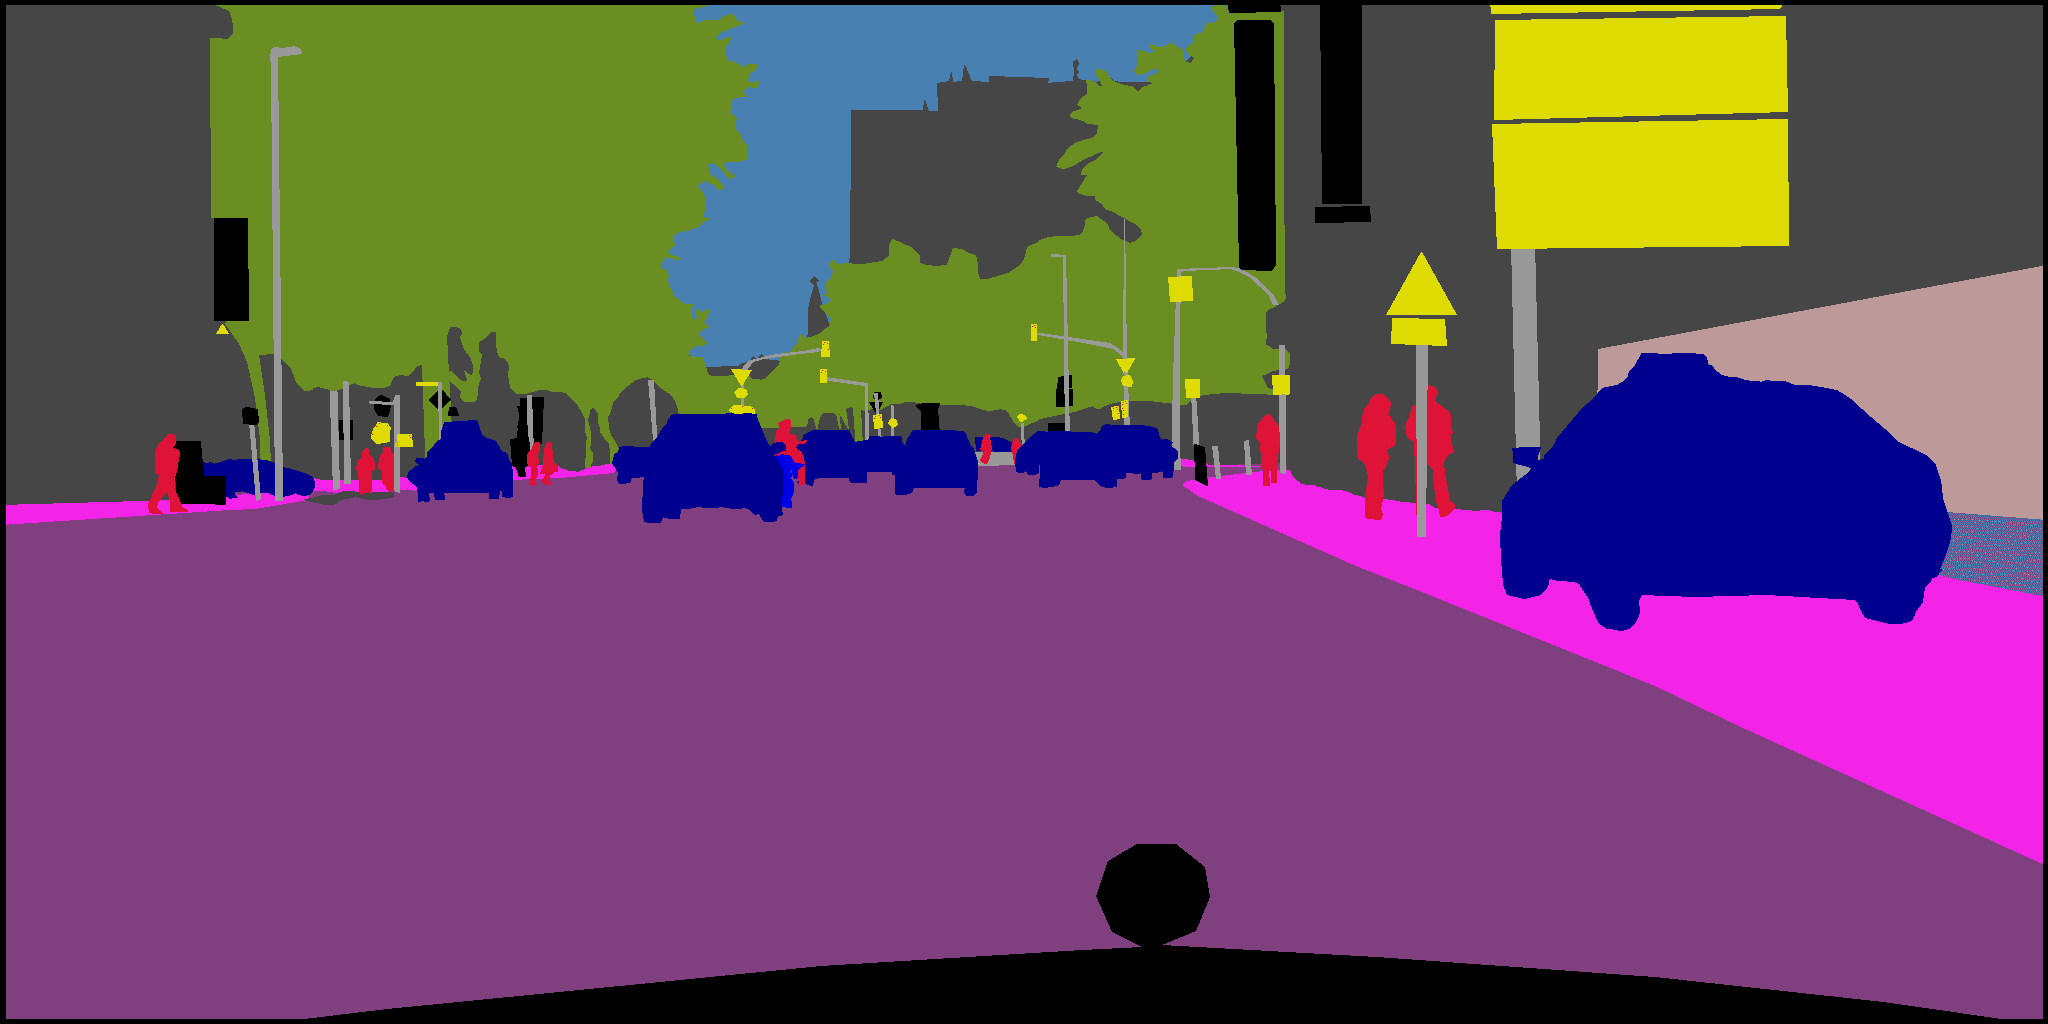
\includegraphics[width=\linewidth, height=0.2\textheight]{Images/Chapter3/aachen_000005_000019_gtFine_color.png}
		\caption{تصویر رنگارنگ}
		\label{f64}
	\end{subfigure}\hfil
	\begin{subfigure}{0.45\textwidth}
		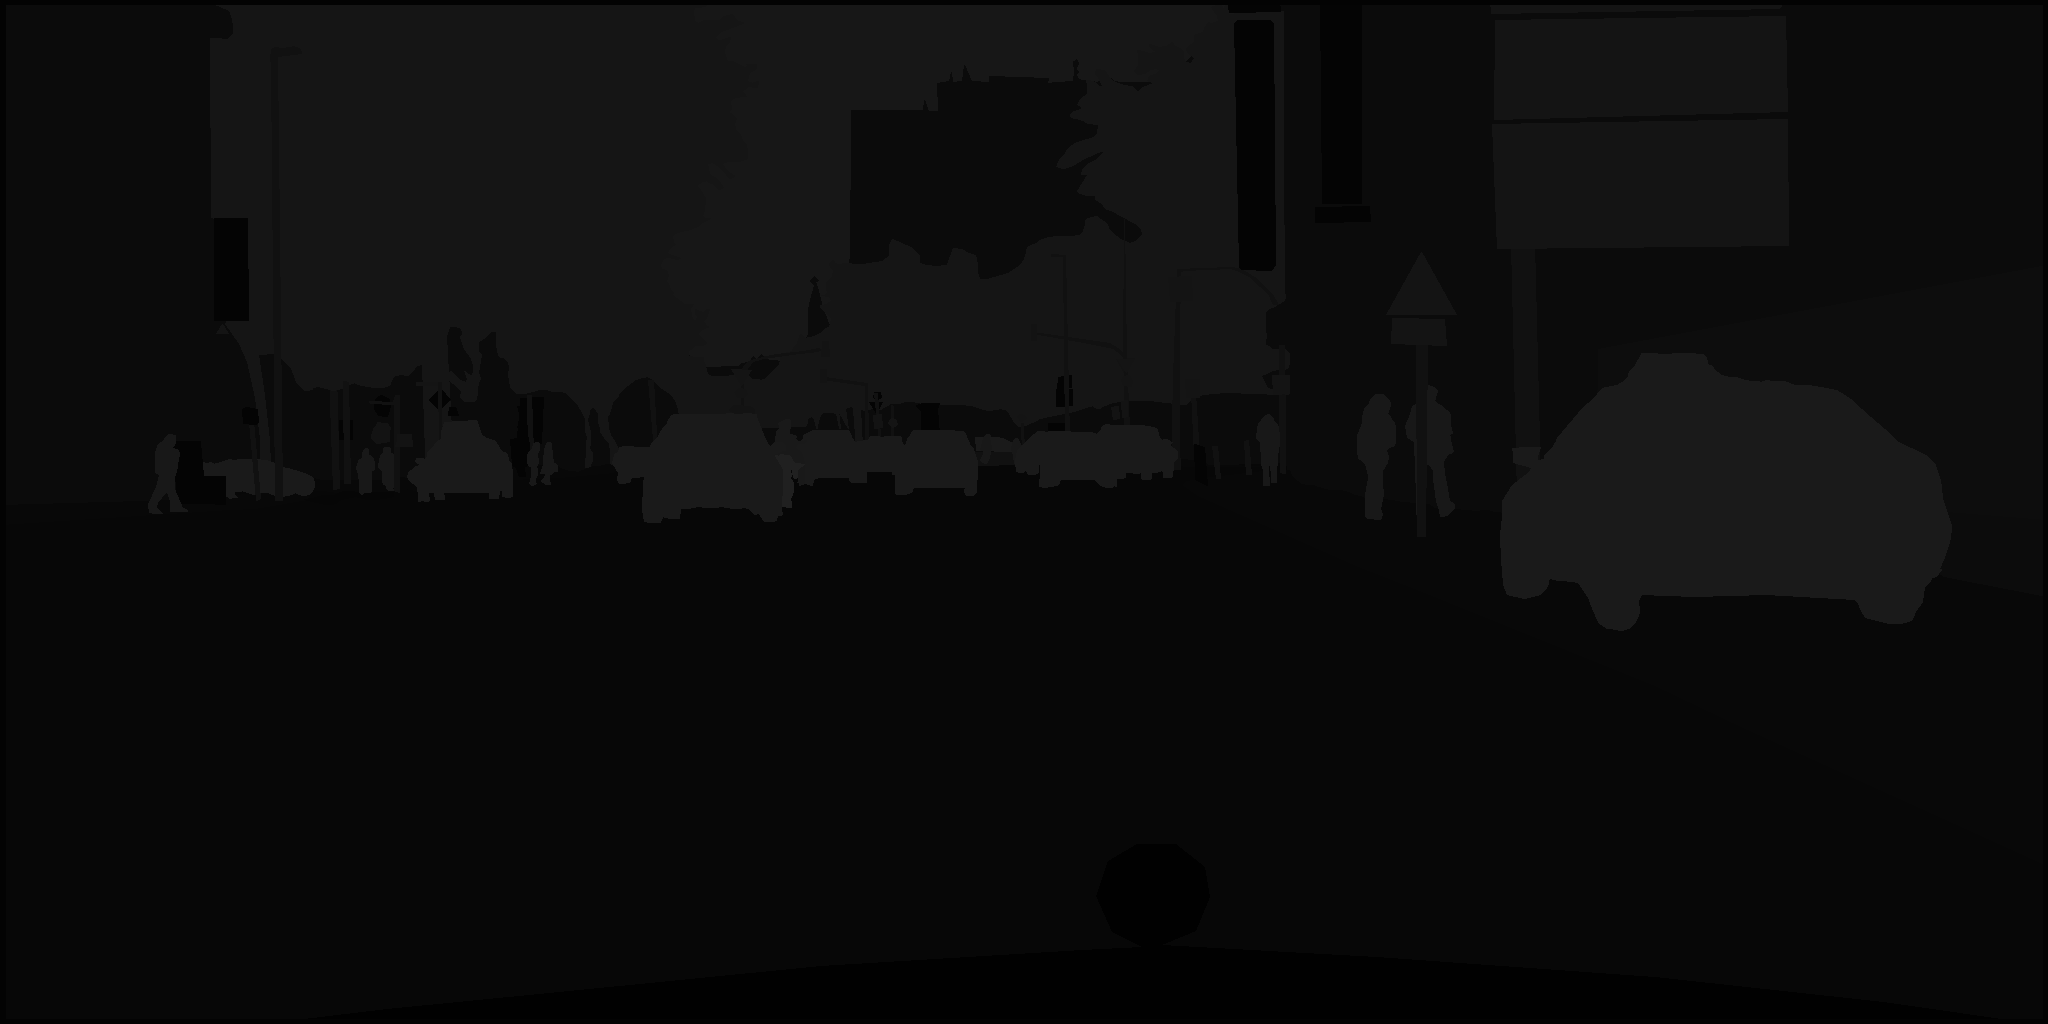
\includegraphics[width=\linewidth, height=0.2\textheight]{Images/Chapter3/aachen_000005_000019_gtFine_labelIds.png}
		\caption{تصویر خاکستری شناسه‌ها}
		\label{f65}
	\end{subfigure}
	\centering
	\caption{نمونه تبدیل نقشه تقسیم‌بندی شده به تصویر رنگارنگ متناظر}
	\label{fig:fig3}
\end{figure}

\section{معماری رمزگذار-رمزگشا}

معماری رمزگذار-رمزگشا
\LTRfootnote{Encoder-decoder}
یک نوع معماری شبکه عصبی است که برای یادگیری توالی به توالی
\LTRfootnote{Sequence to sequence learning}
\cite{sutskever2014sequence}
مورد استفاده قرار می‌گیرد. این معماری شامل دو بخش اصلی، یعنی رمزگذار
\LTRfootnote{Encoder}
و رمزگشا
\LTRfootnote{Decoder}
است که در آن رمزگذار تصویر ورودی را دریافت و پردازش می‌کند تا مجموعه‌ای از بردار‌های ویژگی‌
\LTRfootnote{Feature vectors}
برای تصویر تولید کند. سپس، این بردار‌های ویژگی‌ توسط رمزگشا برای بزرگ‌نمایی تصویر خروجی به اندازه تصویر ورودی استفاده می‌شوند. ایده اصلی پشت این معماری آن است که بتواند یک فرم از داده (در اینجا تصویر) را دریافت کرده و به فرم دیگری (مانند تصویر تقسیم‌بندی معنایی شده معادل) تبدیل کند. با انجام این کار، خودرو قادر خواهد بود که چگونگی ارتباطات بین تصاویر ورودی و خروجی را درک کند.

این معماری می‌تواند در بسیاری از حوزه‌ها مورد استفاده قرار بگیرد، از جمله پردازش تصویر، ترجمه ماشینی
\LTRfootnote{Machine translation}
، تولید متن توسط تصویر
\LTRfootnote{Image to text}
، و غیره. در هر حالت، رمزگذار مسئول استخراج ویژگی‌های مهم از داده ورودی و تولید ویژگی‌های نهان است که اطلاعات اصلی داده را در خود جاسازی می‌کند. سپس، رمزگشا این ویژگی‌های نهان را به فرم دیگری از داده ترجمه می‌کند که معمولاً خروجی مورد نظر است. این معماری به عنوان یکی از روش‌های موثر برای یادگیری مدل‌های پیچیده از داده‌های توالی به توالی شناخته می‌شود و در مسائلی که توالی و ارتباطات بین داده‌ها مهم هستند، بسیار مفید است. در تصویر زیر، این معماری به صورت یک نمودار نشان داده شده است:

\begin{figure}[ht]
	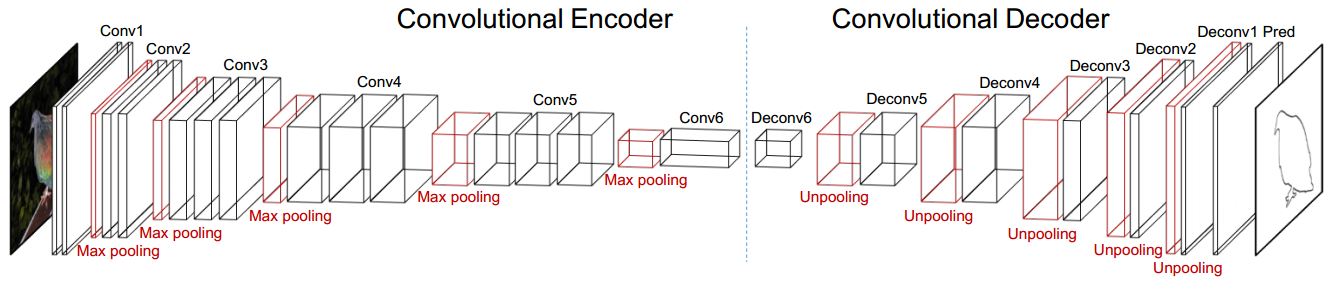
\includegraphics[width=\linewidth, height=0.2\textheight]{Images/Chapter2/encoder-decoder.png}
	\centering
	\caption{معماری رمزگذار-رمزگشا}
	\label{fig:fig4}
\end{figure}

\subsection{شبکه رمزگذار}

رمزگذار، اولین بخش از معماری رمزگذار-رمزگشا است و در پردازش و استخراج اطلاعات از داده ورودی نقش اساسی دارد. این بخش وظیفه استخراج ویژگی‌های معنادار از داده را بر عهده دارد که سپس توسط رمزگشا برای پردازش و بازسازی اطلاعات به فرم دیگر استفاده می‌شود. روشی که فرآیند رمزگذاری کار می‌کند، بسته به نوع کاربرد متفاوت است. در وظایف پردازش تصویر، عموماً از لایه‌های کانولوشنی
\LTRfootnote{Convolutional layers}
به همراه لایه‌های ادغام
\LTRfootnote{Pooling layer}
، فعال‌ساز
\LTRfootnote{Activation function}
و نرمال‌ساز
\LTRfootnote{Normalization}
استفاده می‌شود تا تصویر اصلی به مرور کوچک‌تر شده، اطلاعات اضافی و فضاهای خالی آن حذف شده و در نهایت به تعدادی بردار‌ ویژگی شکسته شود.

لایه‌های کانولوشنی مسئول استخراج ویژگی‌های تصویر ورودی هستند. این لایه‌ها از ویژگی‌های سطح پایین مانند لبه‌ها و رنگ‌ها تا ویژگی‌های سطح بالاتری مانند شکل‌ها و ساختارهای اشیاء را یاد می‌گیرند. هر لایه کانولوشنی مجموعه‌ای از فیلترها را به تصویر ورودی اعمال می‌کند و آن را به بردار‌های ویژگی تبدیل می‌کند که جنبه‌های مختلفی از محتوای تصویر را شامل می‌شود.

لایه‌های ادغام نقشه‌های ویژگی را با حفظ اطلاعات مهم‌تر آن کاهش یا به اصطلاح خلاصه می‌کنند. توابع فعال‌سازی غیرخطی
\LTRfootnote{Non-linear activation functions}
به شبکه این امکان را می‌دهند که روابط پیچیده در داده‌ها آموخته شود. لایه‌های نرمال‌ساز مانند نرمال‌سازی دسته‌ای
\LTRfootnote{Batch normalization}
نیز حساسیت شبکه را به وزن‌های اولیه و نرخ یادگیری
\LTRfootnote{Learning rate}
کاهش می‌دهند و کمک می‌کنند مدل بتواند نرخ‌های یادگیری بالاتری را نیز تحمل کرده و مشکلاتی نظیر انفجار
\LTRfootnote{Exploding gradient descent}
و یا ناپدید شدن گرادیان‌ها
\LTRfootnote{Vanishing gradient descent}
رخ ندهد.

\subsection{شبکه رمزگشا}

رمزگشا، بخش دوم و مهم از معماری رمزگذار-رمزگشا است که مسئول بازسازی بردارهای ویژگی حاصل از رمزگذار و بازسازی آن به شکل اصلی یا شبیه به آن است. این بخش از معماری معمولاً با استفاده از لایه‌های کانولوشنی معکوس
\LTRfootnote{Transposed Convolutional layers}
و یا لایه‌های ادغام معکوس
\LTRfootnote{Unpooling layers}
طراحی می‌شود. برای انجام این کار، باید ارتباطی بین آنچه که رمزگذار شده و آنچه که باید بازسازی شود وجود داشته باشد که عموما در لایه و یا لایه‌هایی بین رمزگذار و رمزگشا به عنوان فضای پنهان
\LTRfootnote{Latent space}
ذخیره می‌شود تا رمزگشا بتواند خروجی معناداری با استفاده از این واحد تولید کند.

از مشکل رایج در معماری رمزگذار-رمزگشا به اندازه بزرگ نبودن فضای پنهان یا بیش از اندازه بزرگ بودن آن است که باعث تولید خروجی ضعیف و یا با جزئیات نامطلوب می‌شود. به عبارت دیگر، اگر فضای پنهان به اندازه کافی بزرگ نباشد، ارتباط بین آنچه رمزگذاری شده و آنچه باید بازسازی شود به طور کامل داخل این ذخیره نشده و در نتیجه نمی‌توان بازسازی معناداری داشته باشیم. در عین حال، اگر فضای پنهان بیش از اندازه بزرگ باشد، الگوهای نامطلوبی توسط مدل کشف شده که متناسب با مساله لزوماً مطلوب ما نیستند.

\section{معماری‌های تقسیم‌بندی معنایی در پزشکی}

در این بخش به مطالعه چند معماری مورد استفاده در مسایل تقسیم بندی معنایی می‌پردازیم.

\subsection{معماری \lr{FCN}}

معماری شبکه کاملا کانولوشنی
\cite{long2015fully}
\LTRfootnote{Fully convolutional network (FCN)}
یک نوآوری بسیار مهم در زمینه تقسیم‌بندی معنایی است که از مدل‌های سنتی شبکه‌های عصبی کانولوشنی با لایه‌های انتهایی کاملا متصل تفاوت دارد. در این معماری، هر پیکسل تصویر به دسته‌های مختلف تقسیم می‌شود، که این امر با استفاده از لایه‌های کانولوشنی و بدون نیاز به لایه‌های کاملاً
\LTRfootnote{Fully connected layer (FC)}
متصل انجام می‌شود. در مدل‌های سنتی‌تر مانند
\verb*|VGG|
\cite{simonyan2014very}
، از لایه‌های کاملاً متصل برای تولید خروجی دسته‌بندی شده استفاده می‌شوند، در حالی که در معماری کاملا کانولوشنی، این لایه‌های کاملاً متصل با لایه‌های کانولوشنی جایگزین می‌شوند. این تغییر باعث می‌شود که شبکه بتواند تصاویر ورودی با ابعاد دلخواه را بپذیرد و خروجی با همان ابعاد تولید کند.

یکی از مزایای این معماری این است که امکان اجرای تقسیم‌بندی معنایی با دقت بالا بدون نیاز به لایه‌های کاملاً متصل فراهم می‌کند. همچنین، اتصالات پرش
\cite{drozdzal2016importance}
\LTRfootnote{Skip Connection}
که در این معماری معرفی شده‌اند، امکان ترکیب اطلاعات معنایی از لایه‌های عمیق با اطلاعات ظاهری از لایه‌های کم عمق را فراهم می‌کنند. این امر منجر به تولید تقسیم‌بندی‌های با جزئیات بیشتر می‌شود که بهبود قابل توجهی در کیفیت و دقت تصویرهای تقسیم‌بندی شده دارد.

\begin{figure}[ht]
	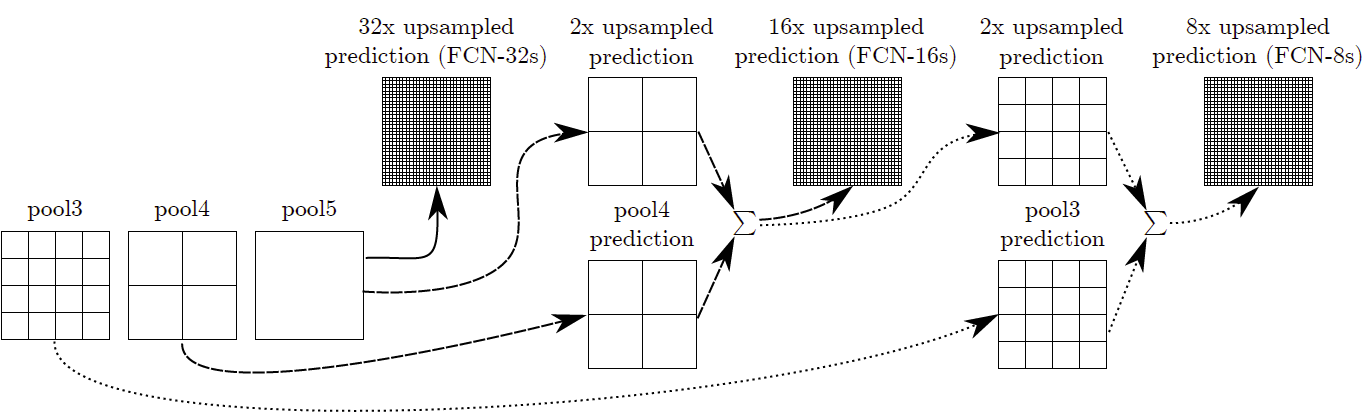
\includegraphics[width=\linewidth, height=0.2\textheight]{Images/Chapter2/FCN.png}
	\centering
	\caption{معماری اتصالات پرش در مدل کاملا کانولوشنی}
	\label{fig:fig5}
\end{figure}

اتصالات پرش یکی از ویژگی‌های کلیدی در شبکه‌های عصبی کانولوشنی
\LTRfootnote{Convolutional Neural Network (CNN)}
هستند که در بسیاری از مسایل تقسیم‌بندی معنایی مورد استفاده قرار می‌گیرند. این اتصالات به شبکه این امکان را می‌دهند که اطلاعات از برخی از لایه‌ها عبور کرده و  مستقیما به لایه‌های بعدی منتقل شوند، در نتیجه جریان مستقیم‌تری از داده دست نخورده به لایه‌های بعدی داشته باشیم.

استفاده همزمان از اتصالات پرش بلند و کوتاه در معماری شبکه‌های عصبی کانولوشنی می‌تواند به بهبود قابل توجهی در دقت تقسیم‌بندی منجر شود. اندازه گام این اتصالات (با اندازه‌های 32، 16 و 8 سلول) مستقیماً بر روی دقت بالانمایی تأثیر می‌گذارد. مدل‌های با گام‌های کوچکتر (در اینجا
\verb*|FCN8|
)، قادرند جزئیات فضایی بیشتری را حفظ کنند و نقشه‌های تقسیم‌بندی دقیق‌تری تولید کنند. اما به همراه این مزیت، گام‌های کوچکتر نیز هزینه محاسباتی
\LTRfootnote{Computational cost}
و زمان استنتاج
\LTRfootnote{Inference time}
را افزایش می‌دهند.

در ارزیابی مدل‌ها با استفاده از شاخص دقت معمولاً مدل‌های با اندازه گام کوچک‌تر عملکرد بهتری را نسبت به مدل‌های مشابه از خود نشان دهند. به عنوان مثال، مدل
\verb*|FCN8|
با مقدار 62.7 در شاخص میانگین اشتراک بر اجتماع
\LTRfootnote{Mean IoU}
عملکرد بهتری را نسبت به مدل‌های مشابه از خود نشان داده می‌دهد.

\subsection{معماری \lr{U-NET}}

معماری
\verb*|U|
-شکل
\cite{ronneberger2015u}
ایده اصلی طرح خود را از شبکه‌های عصبی کانولوشنی می‌گیرد و از آن برای پیش‌بینی پیکسل به پیکسل
\LTRfootnote{Pixel-to-pixel}
در تقسیم‌بندی معنایی استفاده می‌کند. این معماری محدودیت‌های معماری‌های سنتی را برای وظایف تقسیم‌بندی معنایی از بین می‌برد. بر خلاف شبکه‌های عصبی کانولوشنی استاندارد که از لایه‌های کاملاً متصل برای تولید خروجی تصنیفی استفاده می‌کنند، معماری 
\verb*|U|
-شکل، مشابه معماری
\verb*|FCN|
، یک شبکه کاملاً کانولوشنی است که می‌تواند تصاویر ورودی با ابعاد دلخواه را بپذیرد و نقشه‌های تقسیم‌بندی با همان ابعاد تصاویر ورودی را تولید کند.

این مدل نیز از معماری رمزگذار-رمزگشا پیروی کرده که شکلی مانند حرف
\verb*|U|
انگلیسی را تشکیل می‌دهند. در بخش رمزگذار، از کانولوشن‌های تکراری و لایه‌های ادغامی برای یادگیری ویژگی‌های سلسله‌مراتبی استفاده می‌شود. در بخش رمزگشا، ویژگی‌ها بالا‌نمایی می‌شوند و با ویژگی‌های برخی از لایه‌های رمزگذار از طریق اتصالات پرش ترکیب می‌شوند. عموما مدل‌های
\verb*|U|
-شکل از معماری رمزگذار-رمزگشا متقارن
\LTRfootnote{Symmetric encoder-decoder architecture}
\cite{mao2016image}
استفاده می‌کنند که به معنای مشابه بودن این دو بخش دو تعداد لایه‌ها و مشخصات هر لایه بوده، با این تفاوت که عکس یکدیگر عمل می‌کنند.

نوآوری اصلی در معماری
\verb*|U|
-شکل، استفاده کارآمد از اتصالات پرش و توانایی تولید خروجی‌های با وضوح بالا، حتی با مجموعه داده آموزشی نسبتاً کوچک است. اتصالات پرش به شبکه امکان می‌دهند جزئیات ویژگی‌های رمزگذار و رمزگشا را ترکیب کنند و نقشه‌های تقسیم‌بندی دقیق‌تری تولید کنند. این معماری همچنین بازسازی بهتری روی لبه‌های اشیا انجام می‌دهد.

\begin{figure}[ht]
	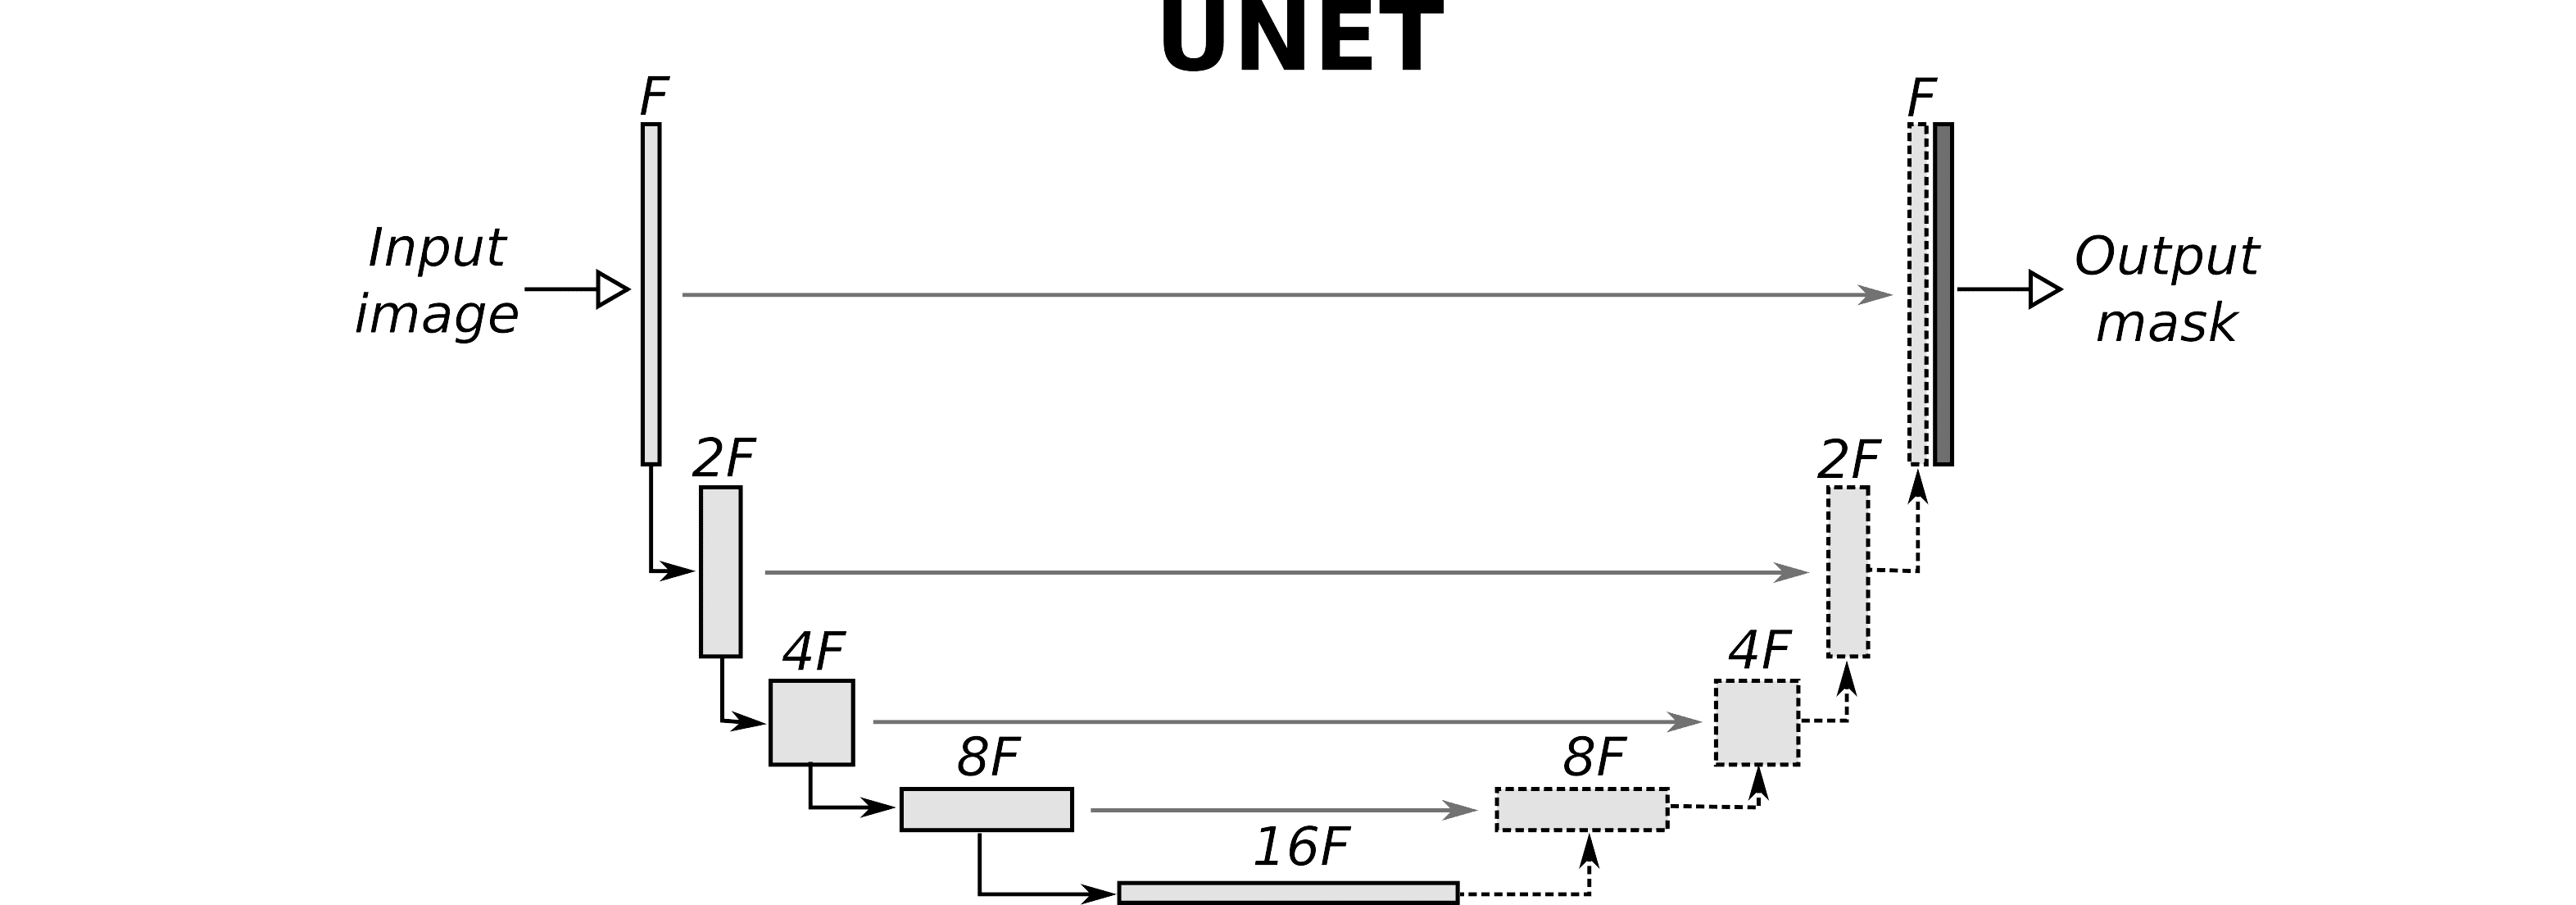
\includegraphics[width=\linewidth, height=0.2\textheight]{Images/Chapter2/UNET.png}
	\centering
	\caption{معماری مدل \lr{U}-شکل}
	\label{fig:fig6}
\end{figure}

\section{خلاصه}

به طور کلی، معماری‌های رمزگذار-رمزگشا به طور قابل توجهی رویکرد حل مسایل تقسیم‌بندی معنایی را تغییر داده‌اند. این معماری‌ها از توانایی‌های شبکه‌های عصبی کانولوشنی برای پیش‌بینی دقیق پیکسل به پیکسل بهره می‌برند و به وجود آوردن نقشه‌های تقسیم‌بندی دقیق و جزئی‌تر کمک می‌کنند. با استفاده از تکنیک‌هایی مانند اتصالات پرش و بالانمایی، ساختار رمزگذار-رمزگشا قادر است جزئیات فضایی و اطلاعات معنایی را با دقت بالاتر در نظر بگیرد و نقشه‌های تقسیم‌بندی دقیق‌تری را تولید کند.
با این حال، معماری‌های
\verb*|FCN|
و
\verb*|U|
-شکل هر کدام ویژگی‌ها و مزایای خود را دارند. معماری U-شکل به دلیل ساختار رمزگذار-رمزگشا تقارنی و استفاده گسترده از اتصالات پرش، نسبت به
\verb*|FCN|
برتری دارد. طراحی منحصر به فرد این مدل به آن امکان می‌دهد که حتی با مجموعه داده‌های آموزشی محدود، خروجی‌های تقسیم‌بندی با وضوح بالا را تولید کند، به‌ ویژه در وظایفی که دقت به جزئیاتی نظیر لبه‌ها حیاتی است، مانند تقسیم‌بندی تصاویر پزشکی. از سوی دیگر،
\verb*|FCN|
رویکردی انعطاف‌پذیرتر را ارائه می‌دهد و ممکن است در مواردی که کارآیی محاسباتی یا مجموعه داده‌های آموزشی بزرگ اولویت دارند، ترجیح داده شود. به طور خلاصه، انتخاب بین این دو معماری بسته به نیازها و شرایط خاص هر پروژه است. با این حال هر دو از سرعت پایینی در زمان استنتاج برخورداند که آن‌ها را برای پردازش لحظه‌ای مناسب نمی‌سازد.

